\documentclass[hyperref={pdfpagelabels=false},ngerman]{beamer}

\usepackage[T1]{fontenc}
\usepackage[utf8]{inputenc}
\usepackage[english]{babel}
\usepackage{lmodern}
\usepackage{graphicx}
\usepackage{amsmath,amssymb,amstext,amsfonts} % mathrsfs
% \usepackage{physics}
\usepackage{booktabs,tabularx}
\usepackage{tikz}
\usetikzlibrary{shapes,calc,arrows,positioning}
\tikzstyle{block} = [rectangle, draw, text width=10em, text centered, minimum height=2em]
\tikzstyle{arrow} = [draw, -latex, thick]
\usepackage{pgfplots}
\pgfplotsset{compat=1.18}
\usepgfplotslibrary{fillbetween,groupplots}
% \usepackage{multirow}
\usepackage{tcolorbox}
\usepackage{pifont}
\usepackage{xspace}
\usepackage{hyperref}
\hypersetup{colorlinks,linkcolor=,urlcolor=blue}

\definecolor{darkgreen}{RGB}{0,176,0}
\definecolor{darkred}{RGB}{200,0,0}
\definecolor{darkyellow}{RGB}{255,165,0}

\newcommand{\cmark}{\ding{51}}%
\newcommand{\xmark}{\ding{55}}%
\newcommand{\fmfvcenter}[1]{\;\vcenter{\hbox{\fmfreuse{#1}}}\;}
\newcommand{\eh}[1]{\,\mathsf{#1}}
\newcommand{\ok}{\textcolor{darkgreen}{\cmark}}
\newcommand{\notok}{\textcolor{red}{\xmark}}
\newcommand{\maybe}{\textcolor{gray}{\cmark}}
\newcommand{\meh}{\textcolor{gray}{\textbf{\huge\lower.1em\hbox{-}}}}
\newcommand{\Lagr}{\mathcal{L}}
\newcommand{\MS}{\ensuremath{M_S}}
\newcommand{\mathi}{\mathsf{i}}
\newcommand{\mycite}[1]{\ensuremath{\text{\textcolor{darkgray}{\tiny [#1]}}}}
\newcommand{\bigcite}[1]{\textcolor{darkgray}{[#1]}}
\newcommand{\dimrep}[1]{\mathbf{#1}}
\newcommand{\dimrepadj}[1]{\mathbf{\overline{#1}}}
\newcommand{\ESSM}{E\textsubscript{6}SSM}
\newcommand{\CESSM}{CE\textsubscript{6}SSM}
\renewcommand{\emph}[1]{\textbf{\textcolor{darkblue}{#1}}}
\newcommand{\myurl}[1]{\href{#1}{#1}}
\newcommand{\Superpot}{\mathcal{W}}
\newcommand{\SuperField}[1]{#1}
\newcommand{\ConjSuperField}[1]{\bar{#1}}
\newcommand{\UY}{\ensuremath{U(1)_{Y}}}
\newcommand{\UN}{\ensuremath{U(1)_{N}}}
\newcommand{\Uem}{\ensuremath{U(1)_\text{em}}}
\newcommand{\SUL}{\ensuremath{SU(2)_\text{L}}}
\newcommand{\SUc}{\ensuremath{SU(3)_\text{c}}}
\newcommand{\SOten}{\ensuremath{{SO(10)}}}
\newcommand{\comma}{,}
\newcommand{\DRbar}{\ensuremath{\overline{\text{DR}}}}
\newcommand{\DRbarp}{\ensuremath{\overline{\text{DR}}'}}
\newcommand{\MSbar}{\ensuremath{\overline{\text{MS}}}}
\newcommand{\SM}{\ensuremath{\text{SM}}}
\newcommand{\MSSM}{\ensuremath{\text{MSSM}}}
\newcommand{\BSM}{\ensuremath{\text{BSM}}}
\newcommand{\EFT}{\ensuremath{\text{EFT}}\xspace}
\newcommand{\THDM}{\ensuremath{\text{2HDM}}\xspace}
\newcommand{\pole}{\ensuremath{\text{pole}}}
\newcommand{\tree}{\ensuremath{\text{tree}}}
\newcommand{\fsstar}{\textbf{*}}
\newcommand{\FS}{\texttt{FlexibleSUSY}\xspace}
\newcommand{\fsh}{\texttt{FS+H}\xspace}
\newcommand{\feft}{\texttt{FlexibleEFTHiggs}\xspace}
\newcommand{\HSSUSY}{\texttt{HSSUSY}\xspace}
\newcommand{\Himalaya}{\texttt{Himalaya}\xspace}
\newcommand{\FH}{\texttt{FeynHiggs}\xspace}
\newcommand{\SPheno}{\texttt{SPheno}\xspace}
\newcommand{\SARAH}{\texttt{SARAH}\xspace}
\newcommand{\SOFTSUSY}{\texttt{SOFTSUSY}\xspace}
\newcommand{\Zv}{\ensuremath{\backslash\mkern-11.0mu{Z_3}}}
\newcommand{\downrightknickarrow}{\mathrel{\scalebox{1.3}{\rotatebox[origin=c]{180}{$\Lsh$}}}}
\newcommand{\threelinebrace}{$\left. \begin{array}{c} \\ \\ \\ \end{array} \right\rbrace$}
\newcommand{\fivelinebrace}{$\left. \begin{array}{c} \\ \\ \\ \\ \\ \end{array} \right\rbrace$}
\newcommand{\twolinebrace}{$\left. \begin{array}{c} \\ \\ \end{array} \right\rbrace$}
\newcommand{\elevenlinebrace}{$\left. \begin{array}{c} \\ \\ \\ \\ \\ \\ \\ \\ \\ \\ \\ \end{array} \right\rbrace$}
\newcommand{\at}{\alpha_t}
\newcommand{\ab}{\alpha_b}
\newcommand{\atau}{\alpha_\tau}
\newcommand{\as}{\alpha_s}
\newcommand{\aem}{\alpha_\text{em}}
\newcommand{\GeV}{\eh{GeV}}
\newcommand{\TeV}{\eh{TeV}}
\newcommand{\Qpole}{\ensuremath{Q_\text{pole}}}
\newcommand{\Qlow}{\ensuremath{Q_\text{low}}}
\newcommand{\Qmatch}{\ensuremath{Q_\text{match}}}
\newcommand{\QTHDM}{\ensuremath{Q_\text{\THDM}}\xspace}
\newcommand{\DMh}{\ensuremath{\Delta M_h^{(\texttt{SS+H})}}}
\newcommand{\DMhQpole}{\ensuremath{\Delta M_h^{(\Qpole)}}}
\newcommand{\DMhQmatch}{\ensuremath{\Delta M_h^{(\Qmatch)}}}
\newcommand{\DMhQlow}{\ensuremath{\Delta M_h^{(\Qlow)}}}
\newcommand{\DMhMt}{\ensuremath{\Delta M_h^{(m_t)}}}
\newcommand{\DMhAlphaS}{\ensuremath{\Delta M_h^{(\as)}}}
\newcommand{\DMhAlphaEm}{\ensuremath{\Delta M_h^{(\aem)}}}
\newcommand{\DMhHSSUSY}{\ensuremath{\Delta M_h^{(\HSSUSY)}}}
\newcommand{\DMhHSSUSYytSM}{\ensuremath{\Delta M_h^{(\hat{y}_t)}}}
\newcommand{\DMhgsMSSM}{\ensuremath{\Delta M_h^{(g_3)}}}
\newcommand{\DMhEFT}{\ensuremath{\Delta M_h^{(v^2/\MS^2)}}}
\newcommand{\DMhFO}{\ensuremath{\Delta M_h^{\text{(FO)}}}}
\newcommand{\Mathematica}{\texttt{Mathematica}}
\newcommand{\Loop}{\ensuremath{\ell}}
\newcommand{\ord}{\ensuremath{\mathcal{O}}}

% set look of slides
\usetheme{Madrid}
\useoutertheme{default}
\useinnertheme{circles}
\usecolortheme{default}
\beamertemplatenavigationsymbolsempty % keine Navigationselemente
\setbeamersize{text margin left = 1cm, text margin right = 1cm}

% define footer
\makeatletter
\setbeamertemplate{footline}
{
  \hfill\hbox{\insertframenumber{} / \inserttotalframenumber\hspace*{4pt}}%
  \vskip3pt%
}
\makeatother
\usecolortheme{tud}

\title{Status of the $M_h$ prediction in the MSSM with FlexibleSUSY}

\author[Alexander Voigt]{Alexander Voigt}

\date{pMSSM topic meeting\\[1em] March 2nd 2026}

% \institute[Aachen]{RWTH Aachen}
\subject{MSSM,Higgs,Supersymmetrie,EFT}
\keywords{MSSM,Higgs,Supersymmetrie,EFT}

%%%%%%%%%%%%%%%%%%%%%%%%%%%%%%%%%%%%%%%%%%%%%%%%%%%%%%%%%%%%%%%%%%%%%%%%%%%%%

\begin{document}

%%%%%%%%%%%%%%%%%%%%%%%%%%%%%%%%%%%%%%%%

\begin{frame}[plain]
  \begin{tikzpicture}[remember picture,overlay]
    \node[anchor=south east] at ([yshift=0.5cm,xshift=-0.5cm]current page.south east) {\includegraphics[width=4cm]{images/RWTH_Logo.pdf}};
    \node[anchor=south west] at ([yshift=0.5cm,xshift=0.5cm]current page.south west) {\includegraphics[width=4cm]{images/FS-logo.png}};
  \end{tikzpicture}
  \titlepage
\end{frame}

%%%%%%%%%%%%%%%%%%%%%%%%%%%%%%%%%%%%%%%%

\begin{frame}{Contents}
  \tableofcontents
\end{frame}

%%%%%%%%%%%%%%%%%%%%%%%%%%%%%%%%%%%%%%%%

\section{Fixed-order calculation}

%%%%%%%%%%%%%%%%%%%%%%%%%%%%%%%%%%%%%%%%%%%%%%%%%%%%%%%%%%%%

\begin{frame}{Contents}
  \tableofcontents[currentsection,currentsubsection]
\end{frame}

%%%%%%%%%%%%%%%%%%%%%%%%%%%%%%%%%%%%%%%%%%%%%%%%%%%%%%%%%%%%

\begin{frame}{Fixed-order calculation (\texttt{NUHMSSMNoFVHimalaya})}
  \emph{Input:} $\aem(M_Z)$, $\as(M_Z)$, $G_F$, $M_Z$, $M_t$, $m_b(m_b)$,\\
  SUSY parameters ($m_{\tilde{f}}^2$, $A_f$, $M_i$, $\mu$, $B\mu$), \ldots
  %
  \begin{center}
    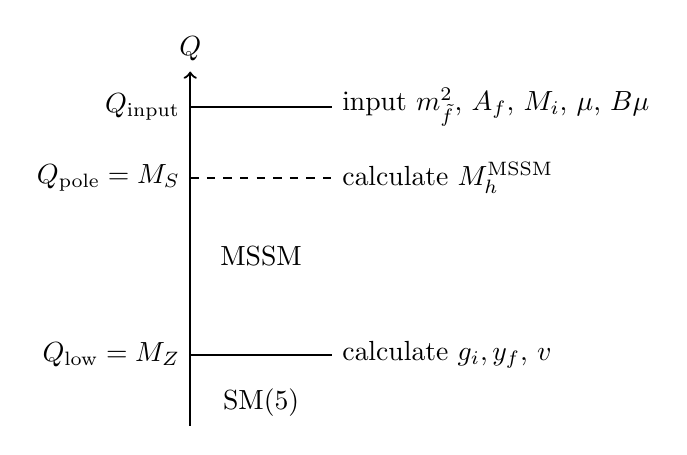
\begin{tikzpicture}[scale=0.9]
      \pgfmathsetmacro{\breite}{2};
      \draw[->, thick] (0,0) -- (0,5) node[above] {$Q$};
      \draw[thick] (0,4.5) node[left]{$Q_\text{input}$} -- ++ (\breite,0) node[right]{input $m_{\tilde{f}}^2$, $A_f$, $M_i$, $\mu$, $B\mu$};
      \draw[thick,dashed] (0,3.5) node[left]{$\Qpole=\MS$} -- ++ (\breite,0) node[right]{calculate $M_h^\MSSM$};
      \draw[thick] (0,1) node[left]{$\Qlow=M_Z$} -- node[above=1cm,black]{MSSM} node[below=0.3cm,black]{SM(5)} ++ (\breite,0) node[right]{calculate $g_i, y_f$, $v$};
    \end{tikzpicture}
  \end{center}
\end{frame}

%%%%%%%%%%%%%%%%%%%%%%%%%%%%%%%%%%%%%%%%%%%%%%%%%%

\begin{frame}{Precision of fixed-order calculation (\texttt{NUHMSSMNoFVHimalaya})}
  \begin{center}
    \begin{tabular}{llll}
      \toprule
      & 1\Loop & 2\Loop & 3\Loop\\
      \midrule
      $y_t$      & full & $y_tg_3^4$ & -- \\
      $y_{b,\tau}$ & full & -- & -- \\
      $g_3$      & full & $g_3^4$ & -- \\
      $g_{1,2}$   & full & -- & -- \\
      $v$        & full & -- & -- \\
      \midrule
      $\beta_{y_t}$    & full & full & full \\
      $\beta_{g_3}$    & full & full & full \\
      $\beta_{\ldots}$    & full & full & full \\
      $\beta_{v_i}$  & full & full & -- \\
      \midrule
      $M_h$  & full & $g_3^2(y_t^4+y_b^4)+(y_t^2+y_b^2)^3+(y_t^2+y_\tau^2)^3$ & $g_3^4 y_t^4$ \\
      \bottomrule
    \end{tabular}
  \end{center}
  % \textcolor{red}{red}: incomplete contributions w.r.t.\ $M_h$
\end{frame}

%%%%%%%%%%%%%%%%%%%%%%%%%%%%%%%%%%%%%%%%%%%%%%%%%%

\begin{frame}{Uncertainty estimate of the fixed-order calculation}
  Possible uncertainty estimates:
  \begin{align*}
    \DMhQpole &= \max_{\Qpole\in[\MS/2,2\MS]}\left|M_h(\Qpole) - M_h(\MS)\right| \\
    \DMhQlow &= \max_{\Qlow\in[M_Z/2,2M_Z]}\left|M_h(\Qlow) - M_h(M_Z)\right| \\
    \DMhgsMSSM &= \left| M_h(g_3^{1\Loop}(M_Z)) - M_h(g_3^{2\Loop}(M_Z)) \right|
  \end{align*}
\end{frame}

%%%%%%%%%%%%%%%%%%%%%%%%%%%%%%%%%%%%%%%%

\section{Pure EFT calculation}

\begin{frame}{Contents}
  \tableofcontents[currentsection,currentsubsection]
\end{frame}

%%%%%%%%%%%%%%%%%%%%%%%%%%%%%%%%%%%%%%%%%%%%%%%%%%

\begin{frame}{Pure EFT calculation (\texttt{HSSUSY})}
  \emph{Input:} same as in fixed-order calculation
  \begin{center}
  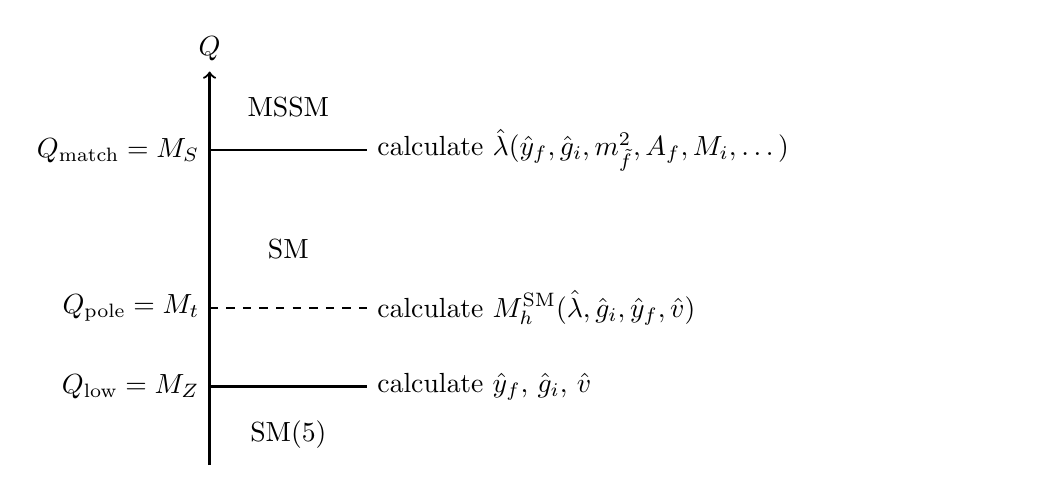
\begin{tikzpicture}
    \pgfmathsetmacro{\breite}{2};
    \draw[->,thick] (0,0) -- (0,5) node[above]{$Q$};
    \draw[thick] (0,4) node[left]{$\Qmatch = \MS$} -- node[above = 0.3cm,black]{MSSM} (\breite,4) node[right,black]{calculate $\hat\lambda(\hat y_f, \hat g_i, m_{\tilde{f}}^2, A_f, M_i,\dotsc)$};
    \draw[thick,dashed] (0,2) node[left]{$\Qpole = M_t$} -- (\breite,2) node[right,black,text width=8cm]{calculate $M_h^\SM(\hat\lambda, \hat g_i, \hat y_f, \hat v)$};
    \draw[thick] (0,1) node[left]{$\Qlow = M_Z$} -- node[above = 1.5cm,black]{SM} node[below = 0.3cm,black]{SM(5)} (\breite,1) node[right,black,text width=8cm]{
      calculate $\hat y_f$, $\hat g_i$, $\hat v$};
    % \draw[<->,blue,thick] (-2.5,1) -- node[above,rotate=90]{RG running} (-2.5,4);
  \end{tikzpicture}
  \end{center}
\end{frame}

%%%%%%%%%%%%%%%%%%%%%%%%%%%%%%%%%%%%%%%%%%%%%%%%%%

\begin{frame}{Pure EFT calculation (\texttt{HSSUSY})}
  \begin{center}
    \resizebox{\textwidth}{!}{%
    \begin{tabular}{lllll}
      \toprule
      & 1\Loop & 2\Loop & 3\Loop & 4\Loop \\
      \midrule
      $\hat\lambda$  & full & $(\hat{y}_t^4+\hat{y}_b^4)\hat{g}_3^2+(\hat{y}_t^4+\hat{y}_b^4+\hat{y}_\tau^4)^2$ & $\hat{y}_t^4\hat{g}_3^4$ & -- \\
      $\hat{v}$        & full & -- & -- & -- \\
      $\hat{y}_t$      & full & $\hat{y}_t\hat{g}_3^4\textcolor{gray}{\,+\,\hat{y}_t^3 \hat{g}_3^2+\hat{y}_t^5}$ & \textcolor{gray}{$\hat{y}_t\hat{g}_3^6$} & $\textcolor{gray}{\hat{y}_t\hat{g}_3^8}$ \\
      $\hat{y}_{b,\tau}$ & full & -- & -- & -- \\
      $\hat{g}_3$      & full & $\hat{g}_3^4$ & $\hat{g}_3^6$ & -- \\
      $\hat{g}_{1,2}$   & full & -- & -- & -- \\
      \midrule
      $\beta_{\hat\lambda}$ & full & full & full & $\hat{y}_t^4\hat{g}_3^6$ \\
      $\beta_{\hat{y}_t}$    & full & full & full & $\hat{y}_t\hat{g}_3^8$ \\
      $\beta_{\hat{g}_3}$    & full & full & full & $\hat{g}_3^{0<n\le 8}$ \\
      $\beta_{\cdots}$  & full & full & full & -- \\
      \midrule
      $M_h$           & full & $(\hat{y}_t^4+\hat{y}_b^4)\hat{g}_3^2+(\hat{y}_t^4 + \hat{y}_b^4)^2$ & $\hat{y}_t^4 \hat{g}_3^4\textcolor{gray}{\,+\,\hat{y}_t^6\hat{g}_3^2+\hat{y}_t^8}$ & \textcolor{gray}{$\hat{y}_t^4 \hat{g}_3^6$} \\
      \bottomrule
    \end{tabular}}
  \end{center}
  \textcolor{gray}{gray}: incomplete contributions w.r.t.\ $M_h$
\end{frame}

%%%%%%%%%%%%%%%%%%%%%%%%%%%%%%%%%%%%%%%%%%%%%%%%%%

\begin{frame}{Uncertainty estimate of the EFT calculation}
  Possible uncertainty estimates:
  \begin{align*}
    \DMhQpole &= \max_{\Qpole\in[M_t/2,2M_t]}\left|M_h(\Qpole) - M_h(M_t)\right| \\
    \DMhQmatch &= \max_{\Qmatch\in[\MS/2,2\MS]}\left|M_h(\Qmatch) - M_h(\MS)\right| \\
    \DMhQlow &= \max_{\Qlow\in[M_Z/2,2M_Z]}\left|M_h(\Qlow) - M_h(M_Z)\right| \\
    \DMhHSSUSYytSM &= \left| M_h(\hat{y}_t^{3\Loop}(M_Z)) - M_h(\hat{y}_t^{4\Loop}(M_Z)) \right| \\
    \DMhEFT &= \left| M_h - M_h(v^2/\MS^2) \right|
  \end{align*}
\end{frame}

%%%%%%%%%%%%%%%%%%%%%%%%%%%%%%%%%%%%%%%%

\section{Hybrid calculation}

\begin{frame}{Contents}
  \tableofcontents[currentsection,currentsubsection]
\end{frame}

%%%%%%%%%%%%%%%%%%%%%%%%%%%%%%%%%%%%%%%%%%%%%%%%%%

\begin{frame}{Hybrid calculation (\texttt{MSSMEFTHiggs})}
  Similar to pure EFT calculation, but $\hat{\lambda}(\Qmatch)$ is
  determined from
  %
  \begin{align*}
    (M_h^2)_{\MSSM}
    &= (M_h^2)_{\SM} \\
    &= \hat{\lambda}(\Qmatch)\hat{v}^2(\Qmatch) + \Delta_{\SM}
  \end{align*}
  $\Rightarrow$
  \begin{align*}
    \hat{\lambda}(\Qmatch)
    = \frac{(M_h^2)_{\MSSM} - \Delta_{\SM}}{\hat{v}^2(\Qmatch)}
  \end{align*}
  %
  \emph{Important:} Loop/coupling expansion on r.h.s.\ required to
  avoid non-cancelled higher-order large logarithms.

  \bigskip

  \emph{Precision:} same as pure EFT calculation, except that series
  of terms of $\ord(v^n/\MS^n)$ is included at $1\Loop$ and $2\Loop$
  level at the respective orders.
\end{frame}

%%%%%%%%%%%%%%%%%%%%%%%%%%%%%%%%%%%%%%%%%%%%%%%%%%

\begin{frame}{Uncertainty estimate of the hybrid calculation}
  Possible uncertainty estimates:
  \begin{align*}
    \DMhQpole &= \max_{\Qpole\in[M_t/2,2M_t]}\left|M_h(\Qpole) - M_h(M_t)\right| \\
    \DMhQmatch &= \max_{\Qmatch\in[\MS/2,2\MS]}\left|M_h(\Qmatch) - M_h(\MS)\right| \\
    \DMhQlow &= \max_{\Qlow\in[M_Z/2,2M_Z]}\left|M_h(\Qlow) - M_h(M_Z)\right| \\
    \DMhHSSUSYytSM &= \left| M_h(\hat{y}_t^{3\Loop}(M_Z)) - M_h(\hat{y}_t^{4\Loop}(M_Z)) \right|
  \end{align*}
\end{frame}

%%%%%%%%%%%%%%%%%%%%%%%%%%%%%%%%%%%%%%%%%%%%%%%%%%

\newcommand{\NUHMSSMNoFVHimalayaMSdata}{data/NUHMSSMNoFVHimalaya_MS-Mh-DMh_TB-20_xt--2.44949.dat}
\newcommand{\NUHMSSMNoFVHimalayaXtdata}{data/NUHMSSMNoFVHimalaya_Xt-Mh-DMh_MS-3000_TB-20.dat}
\newcommand{\HSSUSYMSdata}{data/HSSUSY_MS-Mh-DMh_TB-20_xt--2.44949.dat}
\newcommand{\HSSUSYXtdata}{data/HSSUSY_Xt-Mh-DMh_MS-3000_TB-20.dat}

\begin{frame}{Uncertainty estimate}
  \begin{center}
    \begin{tikzpicture}
      \begin{groupplot}[
        group style={
          group size=1 by 2,
          vertical sep=0,
        },
        height={0.65\textheight},
        width={0.7\textwidth},
        xmode=log,
        log basis x=10,
        xmin=400, xmax=10000,
        legend pos=outer north east,
        legend cell align={left},
        grid
        ]
        \nextgroupplot[
          title={$\tan\beta=20$, $x_t=-\sqrt{6}$},
          ymin=110, ymax=135,
          ytick={115,120,125,130,135},
          ylabel={$M_h$/GeV},
          xticklabels=\empty
        ]
        \addplot[black,thick,densely dotted] table[x index=0, y index=1] {\NUHMSSMNoFVHimalayaMSdata};
        \addlegendentry{FO};
        \addplot[darkgreen,thick,densely dashed] table[x index=0, y index=1] {\HSSUSYMSdata};
        \addlegendentry{EFT};
        \addplot[name path=upper,draw=none] table[x index=0, y expr=\thisrowno{1}+\thisrowno{2}] {\NUHMSSMNoFVHimalayaMSdata};
        \addplot[name path=lower,draw=none] table[x index=0, y expr=\thisrowno{1}-\thisrowno{2}] {\NUHMSSMNoFVHimalayaMSdata};
        \addplot[black!30,fill opacity=0.5] fill between[of=upper and lower];
        %
        \addplot[name path=upper,draw=none] table[x index=0, y expr=\thisrowno{1}+\thisrowno{2}] {\HSSUSYMSdata};
        \addplot[name path=lower,draw=none] table[x index=0, y expr=\thisrowno{1}-\thisrowno{2}] {\HSSUSYMSdata};
        \addplot[darkgreen!30,fill opacity=0.5] fill between[of=upper and lower];
        %%
        \nextgroupplot[height=3cm,ylabel={$\Delta M_h$/GeV},xlabel={$\MS$/GeV},ymin=0,ymax=4,ytick distance=1]
        \addplot[black,thick,densely dotted] table[x index=0,y index=2] {\NUHMSSMNoFVHimalayaMSdata};
        \addplot[darkgreen,thick,densely dashed] table[x index=0,y index=2] {\HSSUSYMSdata};
      \end{groupplot}
    \end{tikzpicture}
  \end{center}
\end{frame}

%%%%%%%%%%%%%%%%%%%%%%%%%%%%%%%%%%%%%%%%%%%%%%%%%%

\begin{frame}{Uncertainty estimate}
  \begin{center}
    \begin{tikzpicture}
      \begin{groupplot}[
        group style={
          group size=1 by 2,
          vertical sep=0,
        },
        height={0.65\textheight},
        width={0.7\textwidth},
        xmin=-3.5, xmax=3.5,
        legend pos=outer north east,
        legend cell align={left},
        grid
        ]
        \nextgroupplot[
          title={$\MS=3$ TeV, $\tan\beta=20$},
          ymin=105,
          ymax=130,
          ytick={110,115,120,125,130},
          ylabel={$M_h$/GeV},
          xticklabels=\empty
        ]
        \addplot[black,thick,densely dotted,restrict x to domain=-3.5:1] table[x index=0, y index=1] {\NUHMSSMNoFVHimalayaXtdata};
        \addlegendentry{FO};
        \addplot[darkgreen,thick,densely dashed] table[x index=0, y index=1] {\HSSUSYXtdata};
        \addlegendentry{EFT};
        \addplot[black,thick,densely dotted,restrict x to domain=1:3.5] table[x index=0, y index=1] {\NUHMSSMNoFVHimalayaXtdata};
        \addplot[name path=upper,draw=none,restrict x to domain=-3.5:1] table[x index=0, y expr=\thisrowno{1}+\thisrowno{2}] {\NUHMSSMNoFVHimalayaXtdata};
        \addplot[name path=lower,draw=none,restrict x to domain=-3.5:1] table[x index=0, y expr=\thisrowno{1}-\thisrowno{2}] {\NUHMSSMNoFVHimalayaXtdata};
        \addplot[black!30,fill opacity=0.5] fill between[of=upper and lower];
        %
        \addplot[name path=upper,draw=none] table[x index=0, y expr=\thisrowno{1}+\thisrowno{2}] {\HSSUSYXtdata};
        \addplot[name path=lower,draw=none] table[x index=0, y expr=\thisrowno{1}-\thisrowno{2}] {\HSSUSYXtdata};
        \addplot[darkgreen!30,fill opacity=0.5] fill between[of=upper and lower];
        %%
        \nextgroupplot[height=3cm,ylabel={$\Delta M_h$/GeV},xlabel={$x_t$ },ymin=0,ymax=3,ytick distance=1]
        \addplot[black,densely dotted,thick,restrict x to domain=-3.5:1] table[x index=0,y index=2] {\NUHMSSMNoFVHimalayaXtdata};
        \addplot[darkgreen,thick,densely dashed] table[x index=0,y index=2] {\HSSUSYXtdata};
      \end{groupplot}
    \end{tikzpicture}
  \end{center}
\end{frame}

\end{document}
